\chapter{Static Analysis Tools}

% TODO: might be worth talking about soundness and completeness

% TODO: https://en.wikipedia.org/wiki/Static_program_analysis Cite an article from here maybe
Static program analysis is the process of automatically analysing source code to extract information about its behavior without executing it \todo{cite}, as opposed to dynamic analysis, which is performed on programs as they are run.
Static analysis tools can ease the burden of software development by automating tasks that would otherwise require manual effort and meticulous attention to detail.
These tools can perform a variety of tasks, ranging from detecting possible bugs \cite{johnson_lint_1978,hovemeyer_finding-bugs_2004} to formal software verification of program properties \cite{blanchet_static-analyzer_2003}.

Static analysis tools are increasingly becoming more important in modern software development, as modern code continues to become more complex and difficult to reason about.
Industry leaders, such as Google \cite{sadowski_analysis-google_2018} and Meta (formerly Facebook) \cite{calcagno_moving-facebook_2015}, have embraced static analysis tools as integral components of their software development workflows.

% TODO: IDE integration

\section{Applications of Static Analysis Tools}
Typically in a software development workflow, multiple static analysis tools are used in conjunction to provide a comprehensive suite of checks.
Often, these tools are integrated into an \textsc{ide} as plugins, allowing them to provide real-time feedback to aid developers in writing idiomatic code.

Refactoring and linting are two major functionalities that these tools provide.
However, because many of these tools include both capabilities, the distinction between them can be blurry.
This section aims to establish definitions for the two terms, which will be used as a basis for subsequent discussion within this thesis.

\subsection{Automated Refactoring}
Code refactoring is a well-established practice in software development.
In his influential book \textit{Refactoring: Improving the Design of Existing Code} \cite{fowler_refactoring_2018}, Fowler defines \textbf{refactoring} as ``the process of changing a software system in such a way that it does not alter the external behavior of the code yet improves its internal structure''.
Refactoring may be employed to eliminate \textbf{code smells}, which are surface indications that could indicate deeper problems in the system.
Code smells are not necessarily problematic on their own, however, they may lead to issues such as bugs or poor maintainability if left unchecked.
Examples of code smells include duplicated code, which can be hard to update without introducing bugs, and long methods, which can be difficult to understand and maintain.
Therefore, it is often productive to refactor code to eliminate code smells, even if the code is still correct and functional.

Static analysis tools can reason about how to safely refactor code in an automated manner, performing refactorings as source-to-source transformations.
These transformations may be implemented as simple text-based replacements or more robust rewrite rules that operate on the abstract syntax tree (\textsc{ast}) of the source code.
% TODO: further discussion of implementation within a different section, when discussing ScalaFix

Automated refactoring support is particularly useful for large codebases, where manual refactoring would be tedious and error-prone.
Generally, when a user makes use of an automated refactoring tool in an \textsc{ide}, they will manually identify the snippet of code that they wish to refactor, and then select the appropriate refactoring from a list of available options.
Fig.~\ref{fig:extract-function-intellij} presents \textit{Extract Method} \cite{fowler_refactoring_2018}, an example of a common refactoring that can be performed automatically on a block code selected by the user.

\begin{figure}[htbp]
  \centering
  \begin{subfigure}{\textwidth}
    \centering
    \begin{minted}[frame=single,highlightlines={4-5},linenos]{scala}
      object Main {
        def main(args: Array[String]): Unit = {
          val bankDetails = getBankDetails()
          println(s"Account name: ${bankDetails.name}")
          println(s"Account balance: ${bankDetails.balance}")
        }
      }
    \end{minted}
    \caption{A snippet of Scala code. A user may wish to extract the highlighted lines into a separate function.}
    \label{fig:extract-function-intellij-before}
  \end{subfigure}
  \begin{subfigure}{\textwidth}
    \centering
    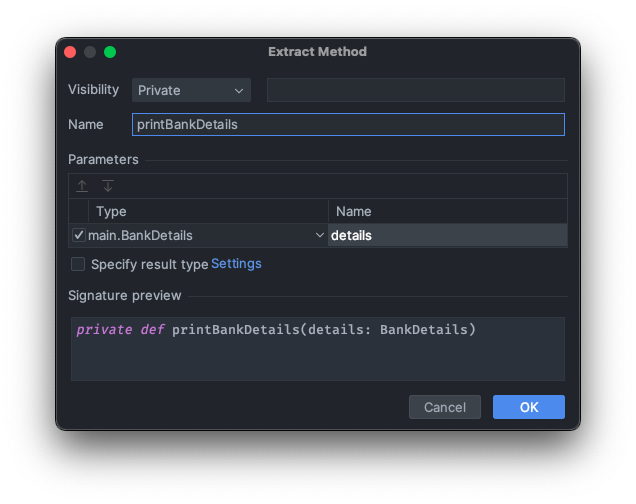
\includegraphics[width=0.75\textwidth]{background/extract-function-intellij.png}
    \caption{When a user selects the highlighted lines from fig.~\ref{fig:extract-function-intellij-before} in IntelliJ IDEA, choosing the \textit{Extract Method} refactoring will open this dialogue to preview changes before applying them.}
    \label{fig:extract-function-intellij-dialogue}
  \end{subfigure}
  \begin{subfigure}{\textwidth}
    \vspace{3ex} % TODO: ew
    \centering
    \begin{minted}[frame=single,highlightlines={4,7-10},linenos]{scala}
      object Main {
        def main(args: Array[String]): Unit = {
          val bankDetails = getBankDetails()
          printBankDetails(bankDetails)
        }

        private def printBankDetails(details: BankDetails): Unit = {
          println(s"Account name: ${details.name}")
          println(s"Account balance: ${details.balance}")
        }
      }
    \end{minted}
    \caption{The result of applying the \textit{Extract Method} refactoring using the chosen parameters in fig.~\ref{fig:extract-function-intellij-dialogue}.}
  \end{subfigure}
  \caption{An example of the \textit{Extract Method} refactoring in IntelliJ IDEA \cite{jetbrains_intellij_2021}.}
  \label{fig:extract-function-intellij}
\end{figure}

\subsection{Linting}
\textbf{Linting} is the process of analysing source code to identify and report issues related to coding style and potential logical errors.
The term originates from the \texttt{lint} program \cite{johnson_lint_1978}, which examined C source code for bugs, as well as wasteful code patterns that may be legal but error-prone.
The tool was also utilised to enforce portability restrictions which aided users in writing portable code that could be compiled on multiple platforms.
Since the release of \texttt{lint}, many linting tools, known as \textbf{linters}, have been developed for a wide range of programming languages.

Linters are provided as standalone tools separate from a compiler, since their primary goal is to suggest improvements for code readability and maintainability, rather than code optimisations.
Modern linters are commonly integrated into \textsc{ide}s, where code analysis performed by the linter is run incrementally in the background.
Any violations found by the linter are displayed directly in the editor as warnings or errors at the relevant locations in the source code.
This provides an ergonomic user experience, as the user can see the results of the analysis in real-time as part of the development workflow.

Furthermore, advanced linters can provide automated code transformations to fix violations which can be corrected automatically by static analysis.
When a linter integrated into an \textsc{ide} reports a warning, it may present the user with a \textit{code action} or \textit{quick fix} to apply the fix automatically.

Many linters are configurable with a set of rules, which specify the types of issues that the linter should detect.
These rules can be enabled or disabled by the user, allowing them to customise the linter to their needs.
Rules can be categorised by their purpose: some rules are concerned with enforcing code style, while others are concerned with detecting code smells or other suspicious code patterns indicative of possible bugs.

\subsubsection{Style checking and code appearance}
% TODO: CheckStyle https://checkstyle.sourceforge.io/, ESLint?
% TODO: https://flake8.pycqa.org/en/latest/   https://peps.python.org/pep-0008/
Linters can be configured to enforce a particular style guide defining a set of conventions for how idiomatic code should be written.
They can highlight style violations and in basic cases, automatically rewrite code to conform to the correct style.
For example, the \textit{Flake8} linter for Python \todo{cite} enforces coding conventions from the PEP 8 style guide \todo{cite}.
Stylistic rules are especially helpful for large projects with multiple contributors, where a consistent coding style can improve readability and maintainability.

\subsubsection{Identifying opportunities for refactoring}
Certain linting rules can aid in the refactoring process by broadly identifying code smells and candidate areas for refactoring, suggesting appropriate actions that the user can take.
As an example, a linter may detect a fragment of code that is repeated in multiple places: this is a code smell, as discussed previously.
The linter may then suggest a code action to automatically apply the \textit{Extract Method} refactoring to avoid code duplication.

\subsubsection{Suggesting idiomatic usage}
Other rules can suggest opportunities to improve more precise snippets of code by utilising language features in a more idiomatic manner.
These rules are especially helpful for new users of a language, who may be unaware of useful language constructs and idioms.
% TODO: Clippy for Rust https://arxiv.org/abs/2310.11738
For example, the \textit{Clippy} linter for Rust \todo{cite article} categorises a collection of rules as \texttt{clippy::complexity} rules to detect code that does something simple in a complex way and suggests a simpler alternative.
Fig.~\ref{fig:hlint-example} provides an example of a similar rule in Haskell, from the \textit{HLint} linter \cite{mitchell_hlint_2024}.
The rule suggests an $\eta$-reduction refactoring, presented to the user as a code action that can be applied automatically.

\begin{figure}[htbp]
  \vspace{3ex} % TODO: make this less hacky
  \centering
  \begin{subfigure}{0.45\textwidth}
    \centering
    \begin{minted}[frame=single]{haskell}
      foo xs = map (+1) xs
    \end{minted}
    \caption{A Haskell function \texttt{foo}, which can be made more concise using $\eta$-reduction.}
  \end{subfigure}
  \hfill
  \begin{subfigure}{0.45\textwidth}
    \centering
    \begin{minted}[frame=single,escapeinside=||]{text}
      Eta reduce
      Found:
        foo xs = map (+ 1) xs
      Why not:
        foo = map (+ 1)
      |\textcolor{gray}{hlint(refact:Eta reduce)}|
    \end{minted}
    \caption{The linter warning shown for \texttt{foo}.}
  \end{subfigure}
  \caption{An example of a warning from the Haskell linter \texttt{hlint}, suggesting a fix that a user can choose to automatically apply.}
  \label{fig:hlint-example}
\end{figure}

Many idiomatic practices exist to avoid common pitfalls that may lead to unintended behaviour.
By highlighting good practices, linters can help users avoid these common mistakes that may cause bugs.
For example, \textit{ESLint} \todo{cite}, one of the most popular JavaScript linters, warns against common JavaScript pitfalls such as using the regular equality operator \texttt{==} instead of its type-safe alternative \texttt{===}.

Linters developed for a specific library provide rules to enforce idiomatic usage specific to the domain of the library.
% TODO: was there a paper that mentioned something like this??? I feel like there was
A library or especially an embedded \textsc{dsl} may require a particular style of usage that is different from the host language.
Therefore, a regular linter for the host language may not be able to detect issues specific to the library.
In this case, an accompanying linter can greatly benefit users: common misuses can be detected and sometimes automatically fixed, and users can be directed to relevant documentation to learn more about correct usage.
For instance, the \textit{xUnit.net} testing framework for C\# is accompanied by an analyser package \cite{xunit_xunitanalyzers_2024} which provides linting rules to enforce best practices specific to xUnit.

\subsubsection{Detecting potential bugs}
Linters may also directly attempt to detect more serious issues in code, such as possible logic errors.
This can be helpful for even experienced users to avoid common pitfalls.
Clippy has \texttt{clippy::suspicious} and \texttt{clippy::correctness} rule categories to identify code that is very likely to be incorrect or useless.
ESLint provides several rules to warn against code patterns that are likely to cause runtime errors, such as re-assigning a \texttt{const} variable.

% TODO: is this needed anymore?
% Given that many linters can perform automated code transformations, the difference between refactoring and linting can be confusing.
% We make the key distinction that linting is concerned with the \textit{detection} of issues in code, while refactoring is concerned with \textit{transforming} code to avoid some of these issues.
% When linters apply automated code transformations to fix issues, some of these transformations may be considered refactorings.
% Thus, many static analysis tools provide both linting and refactoring functionalities.
% For example, when a linter detects a fragment of code that is repeated in multiple places, it may suggest the \textit{Extract Method} refactoring to avoid code duplication.
% The linting tool itself may provide the automated refactoring functionality to perform the transformation.
% The $\eta$-reduction example in fig.~\ref{fig:hlint-example} is another example of a refactoring suggested by a linter to conform to an idiomatic Haskell style.
% We see that \texttt{hlint} can both highlight the issue to the user and perform the suggested refactoring automatically.


% On second thought, this below section seems largely unnecessary and too much of a detour
% \subsection{Bug Fixing and Automated Program Repair}
% * Linters detect code smells which may be indicative of bugs, but don't directly detect bugs
% * Other tools may attempt to detect bugs directly and possibly fix them
% * The difficulty of this depends on the size of the problem space
% * Automated program repair is a growing field of research to identify patches to fix bugs with little to no human intervention
% * Large variety of approaches, many combining static and dynamic analysis techniques
% * Requires fault localisation to identify the locations of bugs
% * Approaches are broadly categorised into heuristic search-based techniques and constraint-based techniques
% * This complexity is due to the huge space of changes to the input source code!
% * However, in a much more limited domain, such as a library, this space is smaller, and much more amenable to automated program repair
% * A large problem as well is that in the vast majority of cases we lack a formal specification for intended program behaviour: that's why we have to rely on tests so many approaches require dynamic analysis too
% * However, in the following sections, we discuss a unique opportunity where this is not the case in the context of parser combinators. So we can just use basic static AST pattern matching techniques

\section{Implementing Static Analysis Tools}
This section first discusses the choices available for implementing a static analysis tool in Scala.
We then discuss how the chosen implementation tool provides a framework for implementing linting and refactoring rules.
% Focus on scala, since we are writing a tool for parsley

% This is traditionally achieved by traversing the \textsc{ast} and pattern matching on the tree structure to identify problematic patterns.
% % TODO: cite https://doc.rust-lang.org/clippy/development/lint_passes.html
% Some linters, such as \texttt{clippy}, are also able to utilise type information from the compiler as part of their analysis.

\chapter{Parser Combinators}
